
\section{Literature Review}
\subsection{Survey on keyless PLS}
\begin{frame}{Wyner's wiretap channel}
\begin{figure}
    \centering
    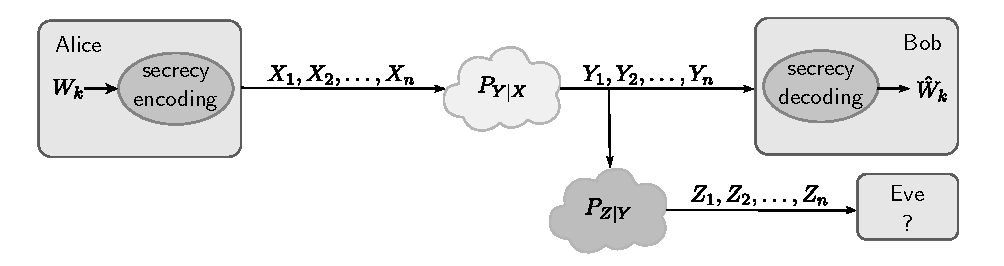
\includegraphics[scale = 0.6]{slides/figures/WiretapChannelWyner.pdf}
    \caption{The wiretap channel as introduced by Wyner in 1975. Perfect secrecy can be achieved without the use of cryptographic keys. }
    \label{fig:wyner}
\end{figure}

\onslide<2->\textbf{Limiting factor}: X-Y-Z form a Markov channel. I.e.: Eve's channel must be a degraded version of Bob's channel.
\end{frame}


\begin{frame}{The generic wiretap channel}
\begin{figure}
    \centering
    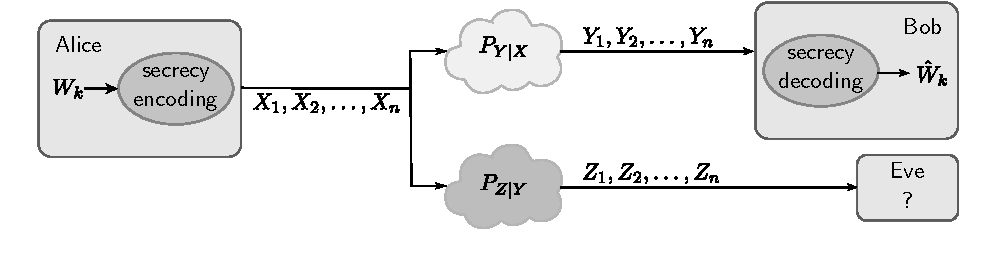
\includegraphics[scale = 0.5]{slides/figures/WiretapChannelCK.pdf}
    \caption{Csisz\'ar and K\"orner generalised Wyner's wiretap channel to include non-degraded wiretap channels.}
    \label{fig:CK}
\end{figure}


\onslide<2-> The generic model matches better the characteristics of the wireless channel.

\onslide<3->Alice transmits opportunistically at times when Bob observes a higher SNR than Eve.
\end{frame}

\begin{frame}{Common Limitations}
\begin{itemize}
    \item Knowledge of the eavesdropper's channel state information (CSI) is needed. 
    \item Secure transmission is possible only when Bob experiences a better signal quality. I.e., a positive secrecy gap is needed.
\end{itemize}

\begin{definition}
    Secrecy gap is the quality difference between the legitimate channel and the wiretap channel. 
\end{definition}

\end{frame}

\begin{frame}{Recent developments}
\begin{itemize}
\item Recent advancements in signalling processing and the employment of multiple-antenna systems  can increase the secrecy gap;

\item Secrecy coding has regained attention and started to expand beyond discrete channel models;

\item Schemes that do not require the eavesdropper’s CSI exist but they are
limited to the case of a single-antenna eavesdropper.
\end{itemize}
    
\end{frame}


\subsection{Survey on key-based PLS}

\begin{frame}{Physical Layer Key Generation}
    \begin{itemize}
        \item A new branch of PLS: key-based PLS, or, \textbf{physical layer key generation};
        \item Aims to generate symmetrical keys, thus enabling upper-layer encryption;
        \item Keys are extracted from the randomness inherited in the wireless multipath channel; 
        \item Early-test bed experimentations prove that physical layer key generation has practical value in today's systems.  
    \end{itemize}
\end{frame}

\begin{frame}{The four stages of physical layer key generation}
    
\begin{figure}
    \centering
    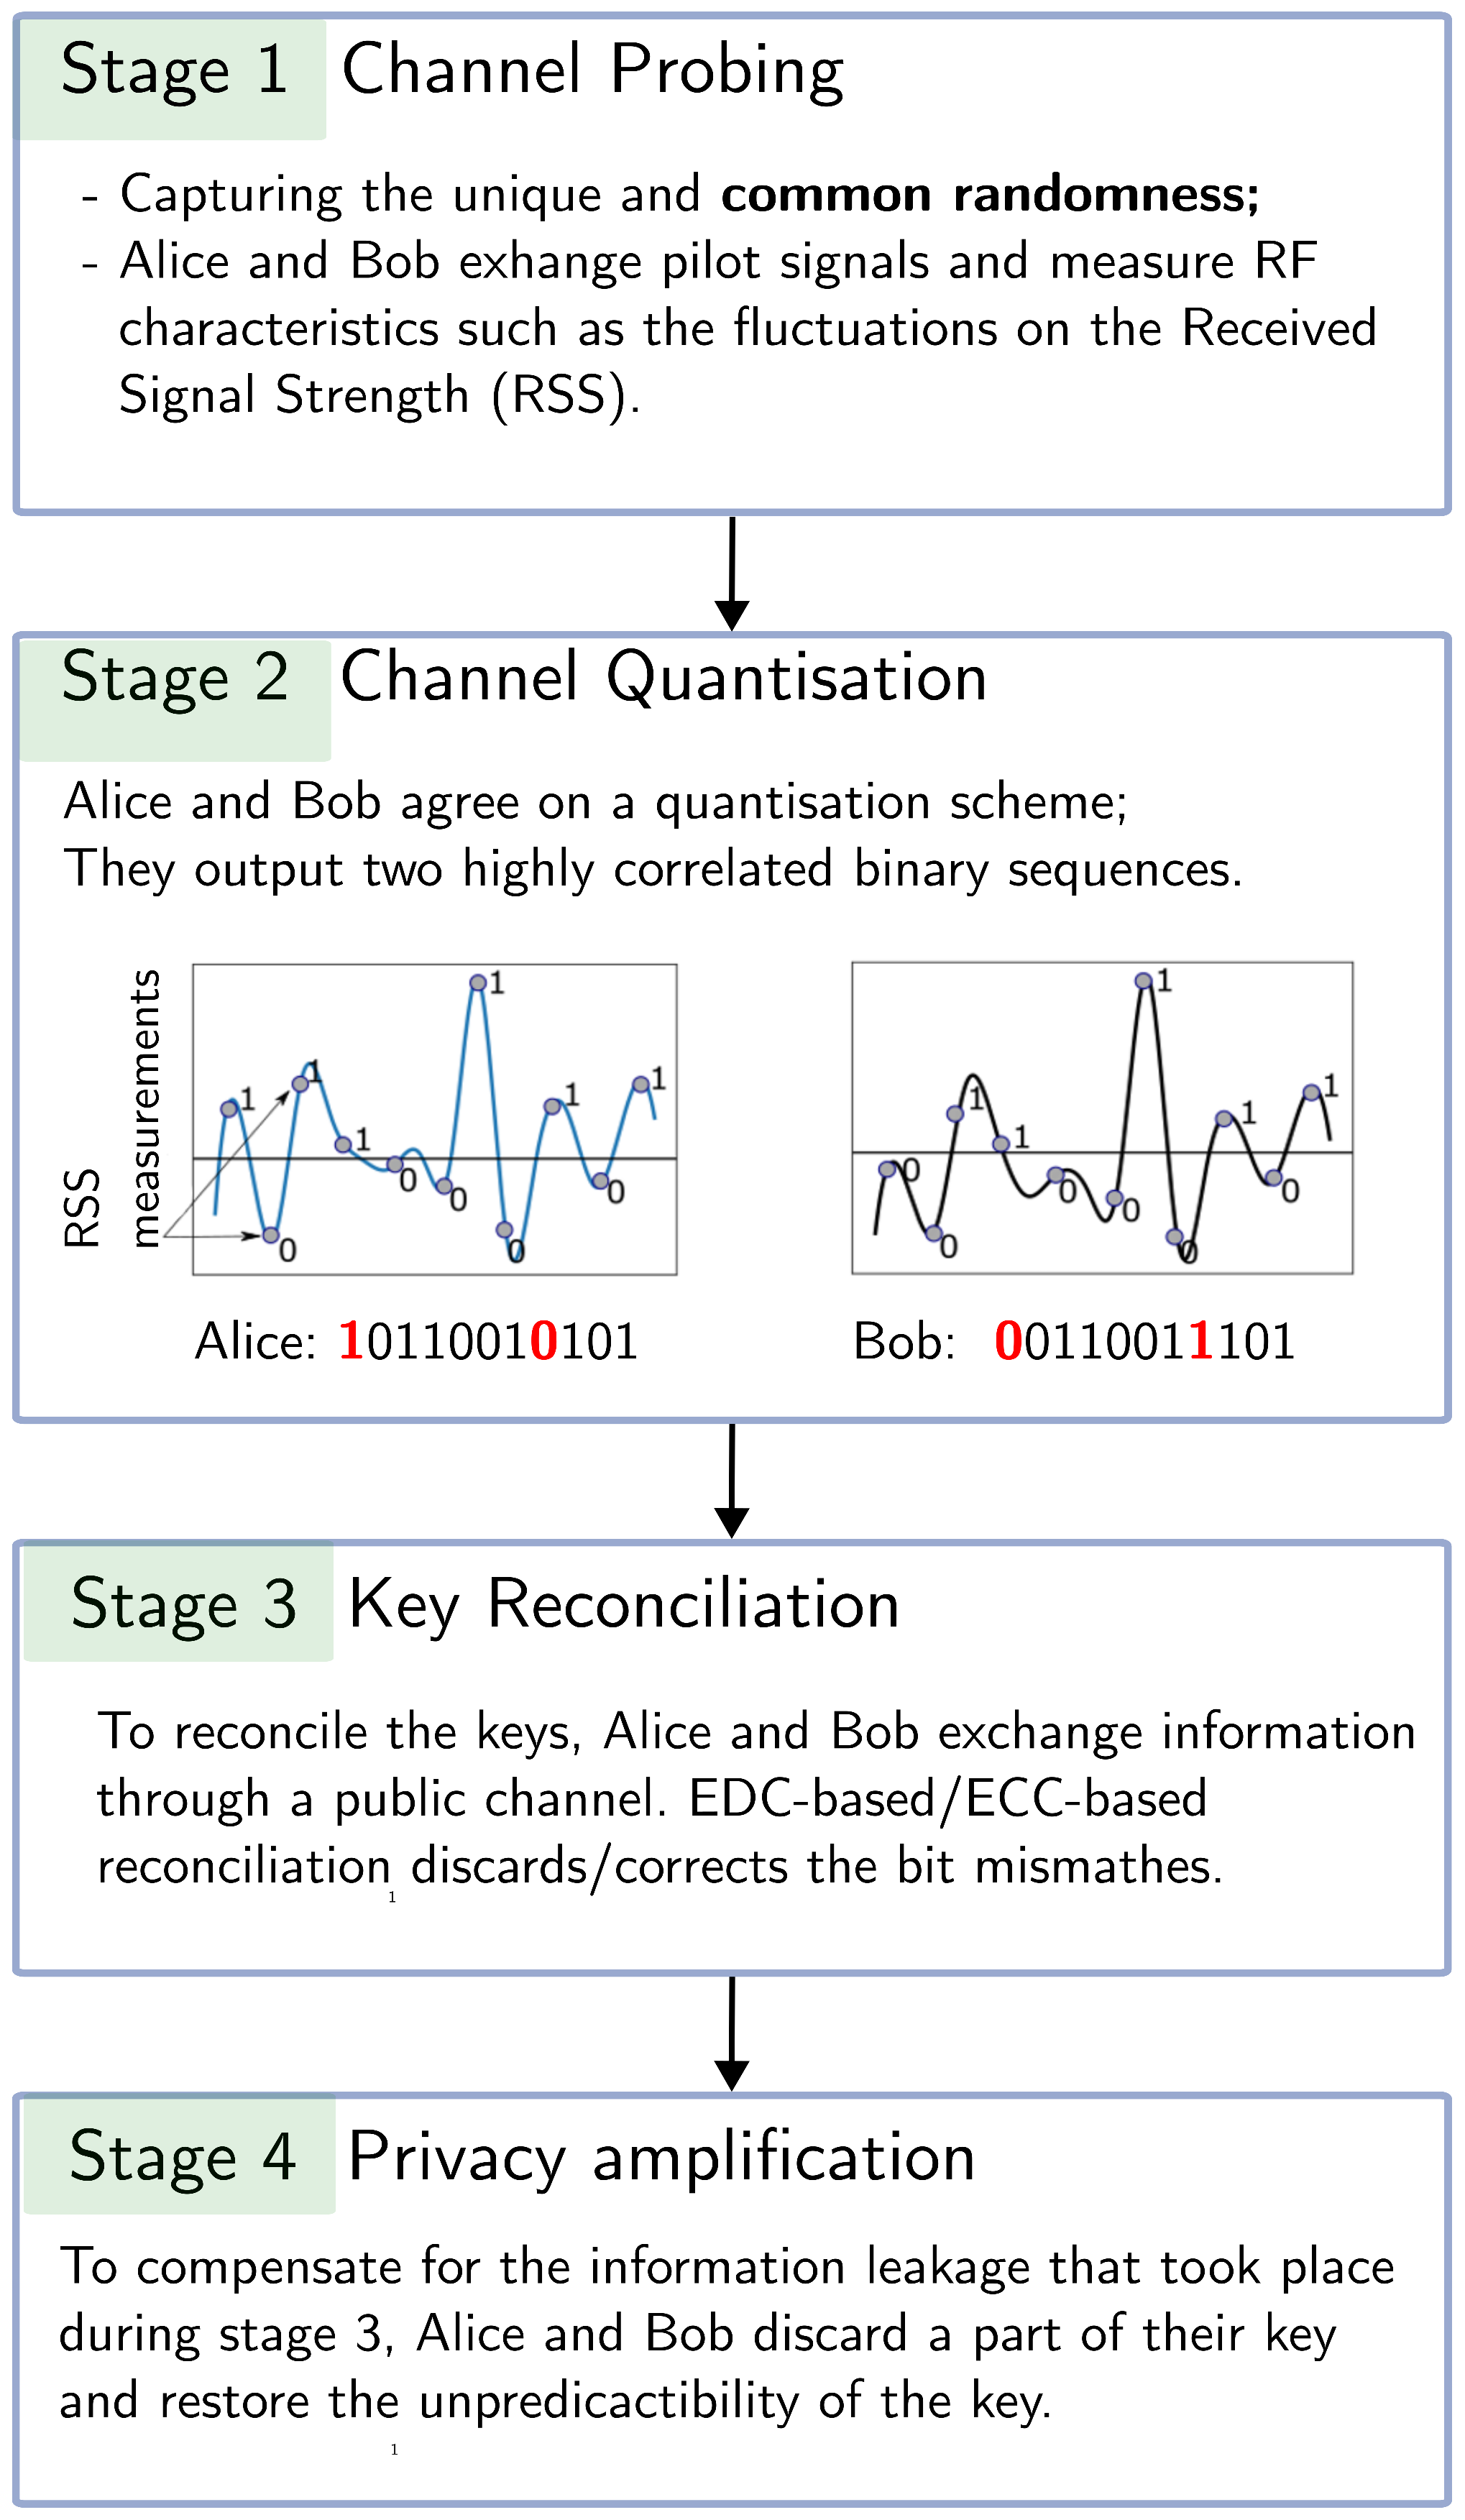
\includegraphics[scale = 0.215]{slides/figures/PLKG.eps}
    \caption{Caption}
    \label{fig:PLKG}
\end{figure}
\end{frame}

\begin{frame}{The four stages of physical layer key generation (cont.)}
    
\begin{figure}
    \centering
    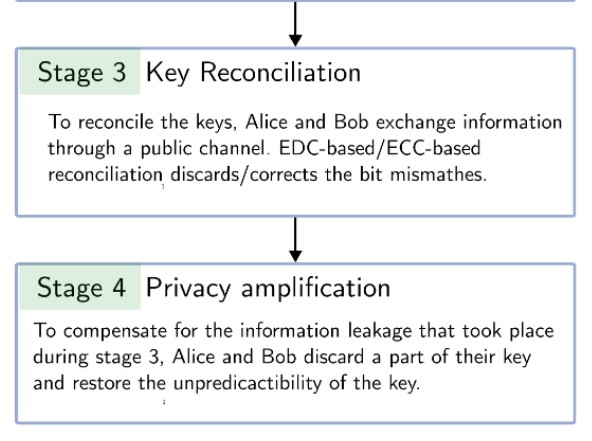
\includegraphics[scale = 0.7]{slides/figures/KGR2.jpg}
    \caption{The four stages of a typical physical layer key generation protocol.}
    \label{fig:PLKG2}
\end{figure}
\end{frame}


\begin{frame}{Limitations of PLKG}
    \begin{itemize}
        \item Low key rates when the wireless channel is not highly dynamic;
        \item Idealistic assumptions:
        \item Key reconciliation may be costly for small devices with little computational capabilities;
        
    \end{itemize}
\end{frame}


\subsection{Survey on physical layer authentication for short-range systems}

\begin{frame}{Authentication}
\begin{figure}
    \hspace*{-2.2cm}
    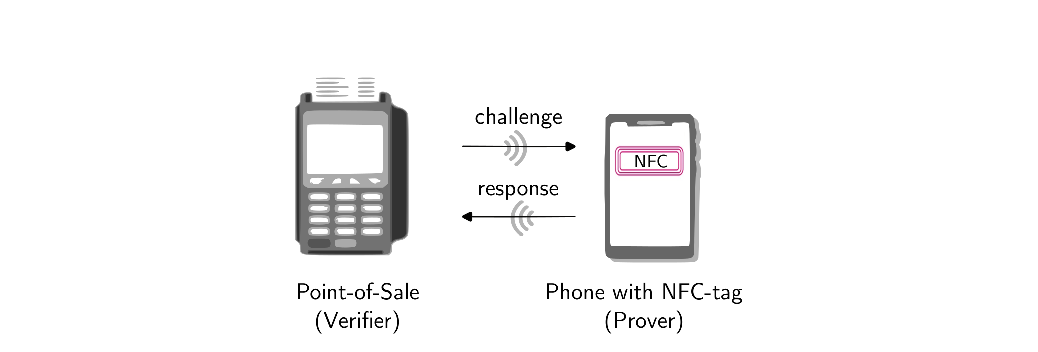
\includegraphics[scale=0.9]{slides/figures/NFC.eps}
    \caption{Verifier-prover example in NFC}
    \label{fig:NFC}
\end{figure}
    
\end{frame}

\begin{frame}{Relay/Replay attacks}
    \begin{figure}
    \hspace*{-1.3cm}
    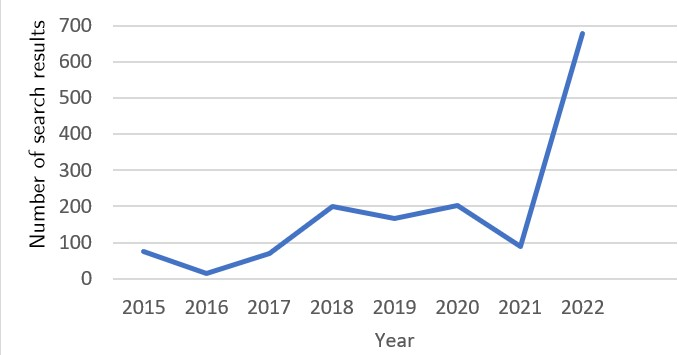
\includegraphics[scale = 0.85]{slides/figures/googleNews.jpg}
    \caption{Number of search results on Google News over the years. Search string: “replay
attacks” OR “relay attacks”}
    \label{fig:google_news}
\end{figure}
\end{frame}

\begin{frame}{Mafia-Fraud}
    \begin{figure}
    \hspace*{-2cm}
        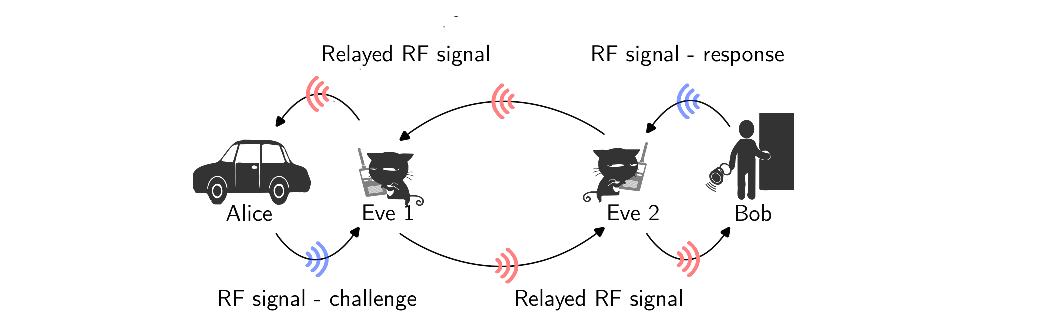
\includegraphics[scale = 0.9]{slides/figures/mafia_fraud.eps}
        \caption{A Mafia Fraud attack with two adversary nodes.}
        \label{fig:enter-label}
    \end{figure}
\end{frame}

\begin{frame}{Terrorist Fraud}
    \begin{figure}
        \centering
        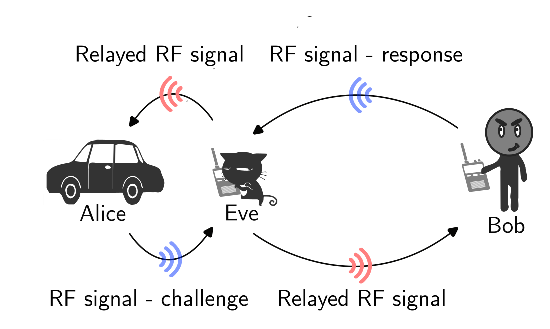
\includegraphics[scale = 0.9]{slides/figures/terrorist_fraud.eps}
        \caption{In a Terrorist Fraud attack, remote Bob cooperates with a local adversary node.}
        \label{fig:enter-label}
    \end{figure}
\end{frame}

\begin{frame}{Current Solutions and Limitations}
    \begin{itemize}
        \item Physical Layer Identification
        \item Time-of-flight distance bounding
        \item Ambient Conditions
        \item RSS and phase-based ranging
    \end{itemize}
    
\end{frame}



%%%%%%%%%%%%%%%%    OLD %%%%%%%%%%%%%%
\iffalse
\begin{frame}
\frametitle{}
\begin{tikzpicture}[snake=zigzag, line before snake = 8mm, line after snake = 8mm]
    % draw horizontal line   
    \draw (0,0) -- (3,0);
    \draw[snake] (3,0) -- (7,0);
    %\draw (4,0) -- (5,0);
    \draw (7,0) -- (10,0);

    % draw vertical lines 1975,1995,2008,today
    \foreach \x in {0,3,7,10}
      \draw (\x cm,3pt) -- (\x cm,-3pt);

    % draw nodes
    \draw (0,0) node[below=3pt] {$ 1975 $} node[above=3pt] {Wyner};
    \draw (1,0) node[below=3pt] {$  $} node[above=3pt] {$ $};
    \draw (2,0) node[below=3pt] {$  $} node[above=15pt] {high interest}
    node[above=7pt] {in academia};
    \draw (3,0) node[below=3pt] {$  1995 $} node[above=3pt] {$  $};
    \draw (4,0) node[below=3pt] {$  $} node[above=3pt] {};
    \draw (5,0) node[below=3pt] {$  $} node[above=3pt] {little interest};
    \draw (6,0) node[below=3pt] {$ $} node[above=3pt] {$  $};
    \draw (7,0) node[below=3pt] {2008} node[above=15pt] {};
     \draw (8,0) node[below=3pt] {$ $} node[above=18pt] {growing interest}
     node[above=7pt]{industry \& academia};
    %\draw (9,0) node[below=3pt] {today} node[above=3pt] {};
    \draw (10,0) node[below=3pt] {today} node[above=3pt] {};
  \end{tikzpicture}
\end{frame}

\fi